\section{Introduction}

  The most prominent component of interior of the Mandlebrot set $M$ is the one bounded by the main cardioid. 
There are infinitely many secondary hyperbolic  components of $\inter M$ attached to it.
In turn, infinitely many  hyperbolic components are attached to each of the secondary components, etc. 
Let us take the union of all hyperbolic components of $\inter M$  obtained this way,
close it up and fill it in (i.e., add all bounded components of its complement%
\footnote{These bounded components could be only queer components of $\inter M$}).
We obtain the set called the {\it molecule} $\MM$ of $M$,
see Figure \ref{molecule}.%
\footnote{It is also called the {\it cactus}.}
In this paper we consider infinitely primitively
renormalizable quadratic polynomials satisfying a {\it molecule condition},
which means that the combinatorics of the primitive renormalization operators involved stays away from 
the molecule (see \S \ref{renorm-sec} for the precise definition in purely combinatorial terms).  


\begin{figure} \label{molecule}
  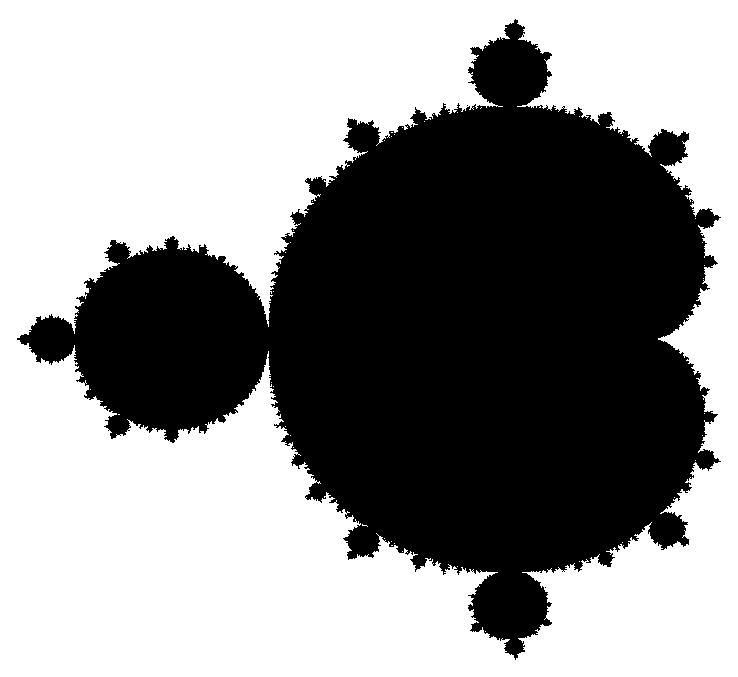
\includegraphics{figures/jeremy-cut.ps}
  \caption{The central molecule of the Mandelbrot set}
\end{figure}

An infinitely renormalizable quadratic map $f$ is said to have {\it a priori bounds}
if its renormalizations can be  represented by quadratic-like maps  $R^n f: U_n'\ra U_n$
with $\mod (U_n\sm U_n')\geq \mu >0$, $n=1,2\dots$.  


Our goal is to prove the following result:

\newtheorem*{Main}{Main Theorem}.
\begin{Main}
  Infinitely renormalizable quadratic maps satisfying the molecule condition have
a priori bounds.
\end{Main}

By \cite{puzzle}, this implies:

\begin{cor}\label{JLC and MLC}  
 Let $f_c: z\mapsto z^2+c$ be an infinitely renormalizable quadratic map satisfying the molecule condition.
Then the Julia set $J(f_c)$ is locally connected, and the Mandelbrot set $M$ is locally connected at $c$.
\end{cor}

Given and $\eta>0$,
let us say that an renormalizable  quadratic map satisfies the $\eta$-{\it molecule} condition
if the combinatorics of the renormalization operators involved stays $\eta$-away from 
the molecule of $\MM$. 
 
In this paper we will deal with the case of renormalizations with sufficiently high periods.
Roughly speaking, we show that if  a quadratic-like map is nearly degenerate 
then its geometry is improving under such a renormalization.
The precise statement requires the notion of  ``pseudo-quadratic-like map'' $f$
defined in  \S \ref{pseudo-puzzle}, and its modulus, $\psimod(f)$.                   %   \note{define}x 

\begin{thm}\label{high periods thm}
 Given  $\eta>0$ and $\rho\in (0,1)$, 
 there exist $\bar\mu>0$ and $\underline p\in \N$ with the following property.  
Let  $f$ be a renormalizable with period $p$ quadratic-like map
satisfying the $\eta$-molecule condition.
If $\psimod(Rf)<\bar\mu$ and $p\geq \underline p$ 
then $\psimod(f) < \rho\, \psimod (Rf)$.
\end{thm} 

The complementary case of ``bounded periods'' is dealt in \cite{K}.
 
\begin{rem}
  Theorem \ref{high periods thm} is proved in a similar way as a more special  result of \cite{decorations}.
The main difference occurs on the top level of the Yoccoz puzzle, which is modified here
so that it is associated with an appropriate periodic point rather than with the fixed point of $f$.%
\footnote{It is similar to the difference between ``non-renormalizable'' and ``not infinitely renormalizable''
cases in the Yoccoz Theorem.} 
We will focus on explaining these new elements, while only outlining the parts
that are similar to \cite{decorations}.     
\end{rem}


Let us now outline the structure of the paper.

In the next section, \S \ref{principal nest}, we lay down the combinatorial framework
for our result, the Yoccoz puzzle associated to dividing cycles, 
and formulate precisely the Molecule Condition. 

In \S \ref{pseudo-puzzle} we summarize necessary background about
{\it pseudo-quadratic-like maps} introduced in \cite{K}, 
and the {\it pseudo-puzzle} introduced in \cite{decorations}.
From now on, the usual puzzle will serve only as a combinatorial frame,
while all the geometric estimates will be made for the pseudo-puzzle.
 Only at the last moment (\S \ref{conclusion})
we return back to the standard quadratic-like context.


In \S \ref{covering lemma sec} we formulate a Transfer Prinsiple,
that will allow us to show that if $\psimod(Rf)$ is small then 
the the pseudo-modulus in between appropriate puzzle pieces is even smaller.

In \S \ref{moduli} we apply the Transfer Principle to the dynamical context.
It implies that the extremal pseuso-distance between two specific parts of the Julia set 
(obtained by removing from the Julia set the central puzzle piece $Y^1$)
is  much bigger than $\psimod(f)$ (provided the renormalization period is big). 
On the other hand, we show that under the Molecule Condition,
this pseudo-distance is comparable with $\psimod(f)$. This yields Theorem \ref{high periods thm}. 
 
\subsection{Terminology and Notation}   
  $\N =\{1,2,\dots\}$ is the set of natural numbers; $\Z_{\geq 0} = \N \cup \{0\}$;
$\D=\{z:\,  |z|<1\}$ is the unit disk, and $\T$ is the unit circle.\\
% $\A(r,R)= \{z: r<|z|<R\}$ is the annulus of modulus $\frac{1}{2\pi} \log (R/r)$;\\
% $\Pi(h)= \{z| 0< \Im z<h\}$ is the horizontal strip.

    A  {\it topological disk} means a simply connected  domain in $\C$.
A {\it continuum} $K$ is a connected closed subset in $\C$. %   containing more than one point.
It is called {\it full} if all components of $\C\sm K$ are unbounded.   
% We say a subset $K$ of a plane is an \fjset\ (for ``filled Julia set'')
% if $K$ is compact, connected, and full.

For subsets $K, Y$ of a topological space $X$,   
notaion $K\Subset Y$ will mean (in a slightly non-standard way) 
that the closure  of $K$ is a compact contained in $\inter Y$.   

  We let $\orb(z)\equiv \orb_g(z)= (g^n z)_{n=0}^\infty$ be the {\it orbit} of $z$ under a map $g$.

  Given a map $g: U\ra V$ and an open topological disk $D\subset V$, 
components of $g^{-1}(D)$ are called {\it pullbacks}  of $D$ under $g$. 
If the disk $D$ is closed, we define pullbacks of $D$ as the closures of the pullbacks of $\inter D$.%
\footnote{Note that the pullbacks of a closed disk $D$ can touch one another, 
so they are not necessarily connected components of $g^{-1}(D)$.} 
In either case, 
given a connected set $X\subset g^{-1}(\inter D)$, we let $g^{-1} (D)|X$ be the pullback of $D$
containing $X$.    

%We let $ x\oplus y = (x^{-1} + y^{-1})^{-1}$ be the {\it harmonic sum} of $x$ and $y$
%(it is conjugate to the ordinary sum by the inversion map $x\mapsto x^{-1}$). 
% Similarly,  $ x\ominus y = (x^{-1} - y^{-1})^{-1}$ stands for the  harmonic difference.


\subsection{Acknowledgement}
We thank Scott Sutherland for help with making Figure \ref{molecule}.
This work has been partially supported by the NSF and NSERC.
